% =================================================================================================
% File:			dp_creazionali.tex
% Description:	Defiinisce la sezione relativa a ...
% Created:		2015-03-26
% Author:		Tesser Paolo
% Email:		tesser.paolo@mashup-unipd.it
% =================================================================================================
% Modification History:
% Version		Modifier Date		Change											Author
% 0.0.1 		2015-03-26 			creato scheltro sezione							Tesser Paolo
% =================================================================================================
% 0.0.2			2015-04-08			inserito scheletro per DP: Prototype e Module	Tesser Paolo
% =================================================================================================
% 0.0.3			2015-04-14			descritto Prototype, Module e Constructor		Tesser Paolo
% =================================================================================================
%

% CONTENUTO DEL CAPITOLO

\subsection{Design pattern creazionali} % (fold)
\label{sub:design_pattern_creazionali}

	\subsubsection{Constructor Pattern} % (fold)
	\label{ssub:constructor_pattern}
		\begin{itemize}
			\item \textbf{Scope dell'utilizzo}: questo pattern è utilizzato per emulare il costruttore tipico della programmazione ad oggetti attraverso delle funzioni che lavorano con gli oggetti;
			\item \textbf{Contesto dell'utilizzo}:
				\begin{itemize}
					\item \textbf{Client}: viene utilizzato in tutte le classi del package \texttt{client::model}. \newline
					Non è possibile fornirne una rappresentazione grafica in quanto questo pattern viene realizzato durante la codifica effettiva delle componenti.
				\end{itemize}
		\end{itemize}
	% subsubsection constructor_pattern (end)

	\subsubsection{Prototype Pattern} % (fold)
	\label{ssub:prototype_pattern}
		\begin{itemize}
			\item \textbf{Scope dell'utilizzo}: questo pattern è utilizzato per generare il meccanismo di ereditarietà tra due classi. Viene anche scelto in modo che i metodi di una classe siano condivisi tra i diversi oggetti in quanto altrimenti, in JavaScript, siccome non è presente il concetto di classi si andrebbe a ripetere un metodo ogni volta che si istanzia un nuovo oggetto e questo non è ottimale;
			\item \textbf{Contesto dell'utilizzo}:
				\begin{itemize}
					\item \textbf{Client}: viene utilizzato nelle classi del package \texttt{client::model} ad esempio tra \texttt{UserModel} e \texttt{UserAdminModel}. \newline
					Non è possibile fornirne una rappresentazione grafica in quanto questo pattern viene realizzato durante la codifica effettiva delle componenti.
				\end{itemize}
		\end{itemize}
	% subsubsection prototype_pattern (end)

	\subsubsection{Module Pattern} % (fold)
	\label{ssub:module_pattern}
		\begin{itemize}
			\item \textbf{Scope dell'utilizzo}: questo pattern serve per garantire, in particolare in JavaScript, l'incapsulamento e la privacy. \'E quindi utilizzato principalmente quando si vuole emulare il concetto di classe, definendo dei membri e dei metodi sia privati che pubblici;
			\item \textbf{Contesto dell'utilizzo}:
				\begin{itemize}
					\item \textbf{Client}: viene utilizzato in tutte le classi del package \texttt{client::model::data} per incapsulare al meglio i membri e i metodi che i modelli dei dati usano. \newline
					Non è possibile fornirne una rappresentazione grafica in quanto questo pattern viene realizzato durante la codifica effettiva delle componenti.
				\end{itemize}
		\end{itemize}
	% subsubsection module_pattern (end)

	\subsubsection{Singleton} % (fold)
	\label{ssub:singleton}
		\begin{itemize}
			\item \textbf{Scope dell'utilizzo}: questo pattern è utilizzato per limitare l'instaziazione di un certo tipo classe ad un solo oggetto in modo tale che esso rimanga unico nel sistema in cui risiede;
			\item \textbf{Contesto dell'utilizzo}:
				\begin{itemize}
					\item \textbf{Client}: viene utilizzato direttamente da AngularJS quando si utilizzano i ``service'' o i ``factory'', utilizzati per creare la logica di business del front-end nel package \texttt{client::model}. Il framework gestisce internamente questo pattern attraverso una hash map che risiede nella cache. Essa rappresenta un singleton manager che detiene le dipendenze che vengono istanziate e le restituisce quando richieste senza crearne una nuova se questa esiste già. \newline
					Non ne viene fornita nessuna rappresentazione grafica in quanto non è una cosa che viene progettata dal team, ma usata direttamente attraverso il framework scelto;
					\item \textbf{Server}: viene utilizzato dalla classe \texttt{server::endpoints::RequestHandler} in quanto quest'ultima, essendo implementata secondo il pattern Front Controller, rappresenta il punto di accesso comune a tutto il sistema in cui confluiscono le richieste provenienti dalle classi appartenenti al package \texttt{server::endpoints} (\ref{ssub:bdsm_app_server_endpoints}). \newline
					\begin{figure}[!htbp]
						\centering
						\centerline{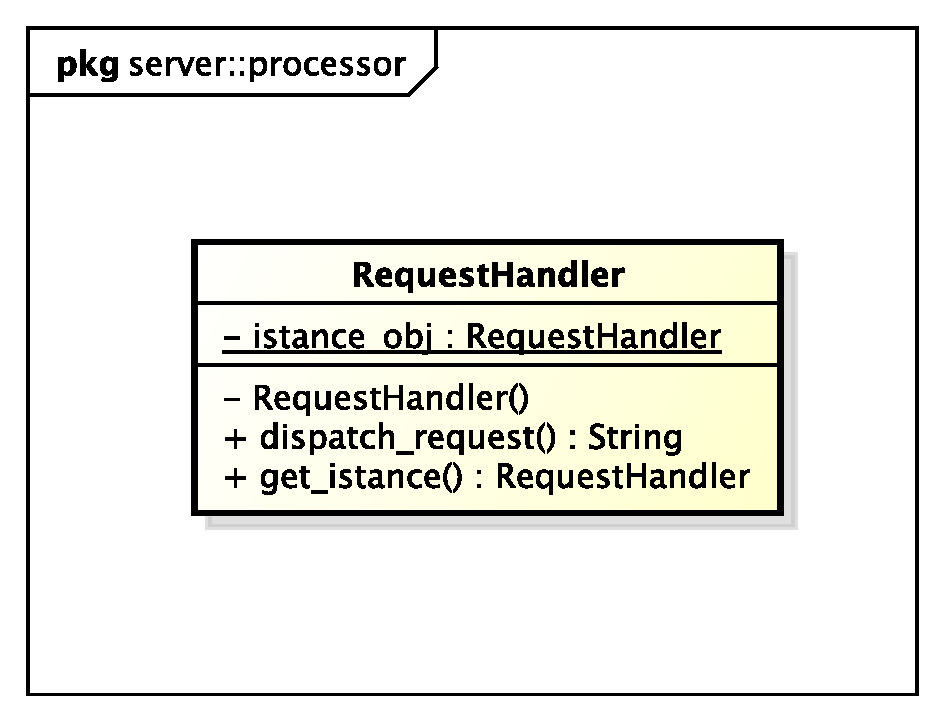
\includegraphics[scale=0.50]{./images/design_pattern_server/dp_singleton.pdf}}
						\caption{Contestualizzazione Singleton - Server}
					\end{figure}
				\end{itemize}
		\end{itemize}
	% subsubsection singleton (end)
% subsection design_pattern_creazionali (end)
